\question{4.14}{Bij een loterij wordt een ronddraaiend rad gebruikt om een winnend nummer te loten. 
Op het rad is een indeling gemaakt in centimeters lopend van $0,00$ tot $100,00$ (wat weer gelijk valt met $0,00$, want de cirkel is dan rond).
De uitkomst van \'e\'en draai met het rad kan men beschouwen als een willekeurige trekking uit de uniforme verdeling tussen $0,00$ en $100,00$.}

\begin{enumerate}[label=(\alph*)]
    \item Hoe groot is de kans dat een willekeurige draai een uitkomst oplevert tussen $40,00$ en $75,00$?
    \answer{
        Bij het rad hebben we te maken met een uniforme verdeling tussen linkergrens $a=0,00$ en rechtergrens $b=100,00$.
        Laat $X$ de kansvariabele zijn die de waarde beschrijft van een draai aan het rad.
        Een uitkomst van deze kansvariabele is een getal $x$ tussen $a$ en $b$.
        Deze uitkomst komt uit een continue kansverdeling, met een kansdichtheidsfunctie (PDF) van
        \[
            f(x) = \begin{cases} \frac{1}{b-a} = \frac{1}{100,00-0,00} = 0,01, & \text{ als } a \le x \le b\\
                                 0,                                              & \text{ anders.}   
            \end{cases}  
        \]
        \begin{center}
            \resizebox{0.9\textwidth}{!}{
                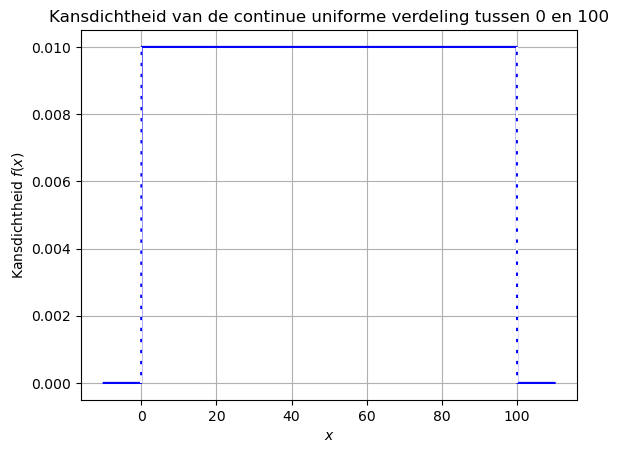
\includegraphics{opg4.14a_1.png}
            }
        \end{center}
        De cumulatieve verdelingsfunctie (CDF) van de uniforme verdeling tussen $a$ en $b$ laat zich beschrijven door
        \[
            F(x) = P(X\le x)=\begin{cases} 0, & \text{ als } x < a\\ \frac{x-a}{b-a}, &\text{ als } a \le x < b\\ 1, & \text{ als } x \ge b \end{cases}
        \]
        \begin{center}
            \resizebox{0.9\textwidth}{!}{
                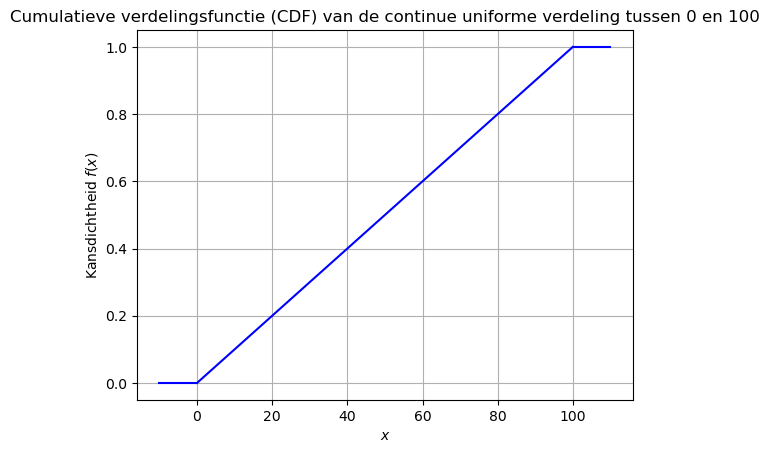
\includegraphics{opg4.14a_2.png}
            }
        \end{center} 
        De kans op een uitkomst tussen $40,00$ en $75,00$ is dus 
        \begin{align*}
            P(40,00 \le X \le 75,00)    &= F(75,00) - F(40,00)\\
                                        &= \frac{75,00 - 0,00}{100,00-0,00} - \frac{40,00 - 0,00}{100,00-0,00}\\
                                        &= 0,75 - 0,40 \\
                                        &= 0,35
        \end{align*}
    }

    \item Hoe groot is de kans dat drie draaien achter elkaar alle drie een uitkomst opleveren tussen $80,00$ en $100,00$?
    \answer{
        De kans dat een draai een uitkomst oplevert tussen $80,00$ en $100,00$ is gelijk aan
        \begin{align*}
            P(80,00 \le X \le 100,00)   &= F(100,00) - F(80,00) \\
                                        &= 1 - \frac{80,00-0,00}{100,00-0,00} \\
                                        &= 1 - 0,80 = 0,20
        \end{align*}
        Aangezien afzonderlijke draaien onafhankelijk zijn van elkaar (de uitkomst van de eerste draai beinvloedt niet de kansen van latere draaien) is de kans
        op drie keer een draai tussen $80,00$ en $100,00$ gelijk aan $0,20 \cdot 0,20 \cdot 0,20 = 0,008$.
    }

    \item We doen twee draaien met het rad. Hoe groot is de kans dat de eerste draai een uitkomst kleiner dan 20,00 oplevert en de tweede draai een uitkomst groter dan $20,00$?
    \answer{
        Deze kans is gelijk aan 
        \begin{align*}
            P(X < 20,00) \cdot P(X > 20,00)  &= 0,2 \cdot 0,8 = 0,16.
        \end{align*} 
    }

    \item Gegeven is dat de eerste draai $60$ oplevert, hoe groot is dan de kans dat de tweede draai een groter getal oplevert?
    \answer{
        Omdat de uitkomsten van opeenvolgende draaien onafhankelijk zijn van elkaar, is de kans dat de tweede draai een groter getal oplevert gelijk aan
        \[
            P(X\ge 60) = P(60 \le X \le 100,00) = F(100,00) - F(60) = 1 - 0,6 = 0,4
        \]
    }
    
    \item Gegeven is dat de eerste draai $A$ oplevert, hoe groot is dan de kans dat de tweede draai meer dan $A$ oplevert?
    \answer{
        Als de eerste draai de waarde $A$ oplevert, dan is de kans dat de tweede draai meer oplevert gelijk aan
        \begin{align*}
            P(X > A)    &= P(A \le X \le 100,00) \\
                        &= F(100,00) - F(A) \\
                        &= 1 - \frac{A-0,00}{100,00-0,00} \\
                        &= \frac{100,00-A}{100,00}
        \end{align*}
    }

\end{enumerate}